\chapter{Aritmetica dei calcolatori}

\section{Informazione nei computer}

\subsection{I transistor}
\begin{wrapfigure}{r}{0.4\textwidth}
	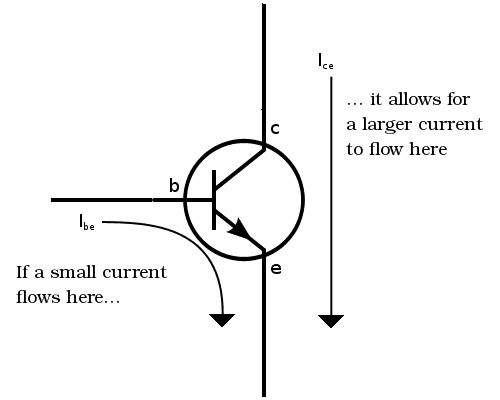
\includegraphics[width=0.9\linewidth]{images/transistor.png}
	\label{fig:transistor}
	\centering
\end{wrapfigure}
Tutti i computer moderni sono composti da \textit{transistor} (detti anche triodi) che sono strutture bistabili, ovvero che possono assumere due stati come un interruttore: 0=spento e 1=acceso. Molti \textit{transistor} collegati tra loro in una sorta di matrice possono rappresentare delle serie di porte logiche, ed è questa la struttura che sta alla base dell'architettura dei moderni calcolatori.\\ 
Un computer memorizza (e manipola) solo sequenze di 0 e 1 (sequenze di bit); anche l’ENIAC funzionava allo stesso modo, solo che al posto dei \textit{transistor} era composto da \textit{valvole termoioniche}, che in ultima analisi non erano differenti nel funzionamento (assumono sempre i due stati descritti in precedenza, solo più lentamente).
\subsection{Interpretazione delle informazioni} In seguito le sequenze di bit che i computer elaborano/memorizzano possono essere interpretate in tantissimi modi diversi, tra cui numeri, caratteri, suoni, immagini, istruzioni e molti altri.\\
Alla base di tutte le interpretazioni che si possono dare alle stringhe di simboli (che nel caso del computer sono proprio i due stati del bit) sta il concetto di \textbf{codifica}. La \textbf{codifica} è appunto uno schema, una legge, un \textit{mapping} che permette di tradurre prima ed interpretare poi stringhe di simboli.
Nell’ambito dell’IT le codifiche sono fortemente caratterizzate dalla lunghezza (dal numero di bit) delle “parole” elementari della codifica. Ad esempio per rappresentare tutti i caratteri (tabella ASCII) utilizziamo  8 bit [256 caratteri].
Si osservi che essendo i \textit{transistor} sistemi bistabili la base 2 (con cifre 0 e 1) è perfetta per rappresentare la codifica dei dati memorizzati/elaborati da essi.
\section{I numeri}
Limitiamoci al caso dei numeri per spiegare il concetto di \textbf{codifica}:\\
Ricordiamo che i  metodi di rappresentazione numerica che studiamo sono posizionali, ovvero il peso di ogni cifra varia in base alla posizione che essa  occupa.\\
In generale se una base è composta da B elementi essa ha B cifre (da 0 a B-1) utilizzate per scrivere ogni numero.
Questa formula ci restituisce il valore di ogni numero scritto in una qualsiasi base B:\\
\[c_{i} c_{i-1} c_{i-2}... c_{0}=c_{i}*B^{i}+...+c_{0}*B^{0}\]\\
dove $c_{i}$ è la cifra in posizione \textit{i}.

\subsection{Regole di conversione tra basi}
\textit{(un elenco delle principali basi è troppo mainstream?)}\\\\
Vediamo ora come operare la conversione tra le principali basi:
\begin{itemize}[noitemsep,nolistsep]
	\item \textbf{da base 2 a base 16}: partendo da destra, si dividono le cifre binarie in gruppi da 4 cifre ciascuno, e ognuno di questi corrisponderà a una cifra esadecimale;
	\item \textbf{da base 2 a base 8}: analogamente, si dividano le cifre binarie in gruppi da 3 cifre ciascuno, e ognuno di questi corrisponderà a una cifra ottale;
	\item \textbf{da una qualsiasi base $B$ a base 10}: come visto sopra, si moltiplica ogni cifra $c_{i}$ per $B^{i}$, dipendentemente dalla sua posizione;
	\item \textbf{da base 10 a una qualsiasi base B}:
	\begin{enumerate}[noitemsep,nolistsep]
		\item si consideri un numero $x_{10}$ e una base $B$;
		\item si divida $x$ per $B$;
		\item il resto della divisione è la cifra da inserire a sinistra nel numero convertito;
		\item si assegni a $x$ il quoziente della divisione;
		\item si torni al punto 2 e si ripeta finché $x>B$.
	\end{enumerate}
\end{itemize}
\begin{figure}[H]
	\centering
	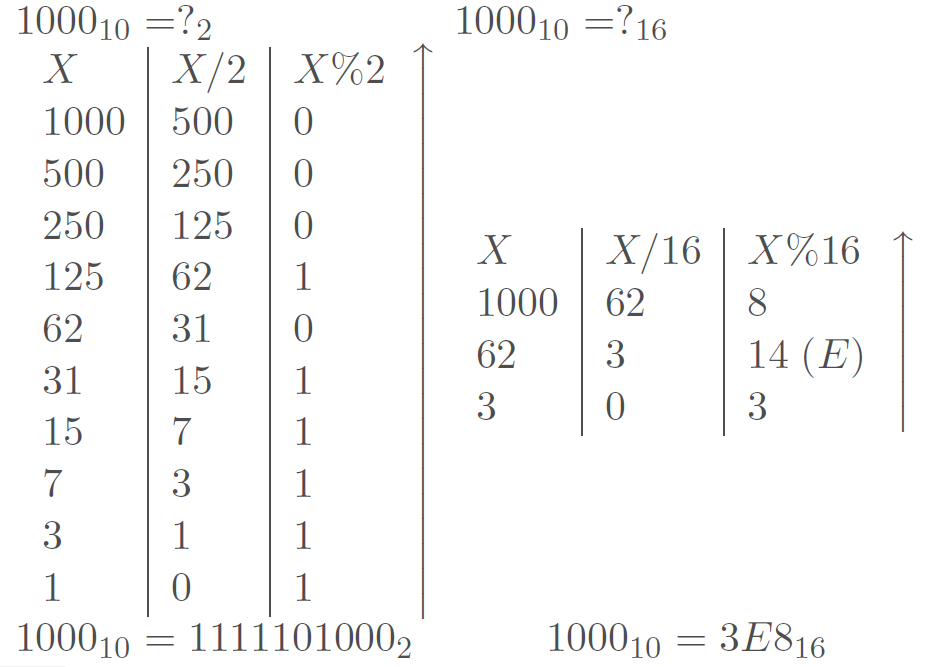
\includegraphics[width=0.7\textwidth,keepaspectratio]{images/esempi_conversioni.png}
	\caption{Alcuni esempi di conversione}
\end{figure}

\subsection{I naturali} Nella codifica binaria un numero naturale è rappresentato su \textit{k} cifre binarie, dove con \textit{k} cifre si possono rappresentare i numeri tra 0 e $2^{k}-1$.\\
La codifica più comune per gli interi spesso usa i byte, sequenze di 8 bit, che tuttavia richiedono molte cifre per rappresentare un numero e quindi spesso, per semplificare la lettura, si usa scrivere i numeri in esadecimale (quindi scrivendo un quarto delle cifre rispetto alla binaria).

\paragraph*{Somma e sottrazione}
Le operazioni somma e sottrazione funzionano allo stesso modo del sistema utilizzato nella numerazione decimale con il riporto. Si guardino gli esempi qui sotto riportati, già di per sè esplicativi del processo:\\
\begin{figure}[H]
	\centering
	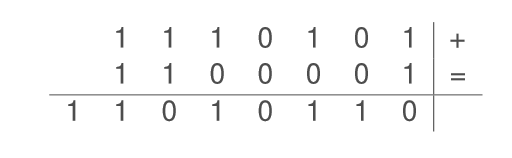
\includegraphics[width=0.6\textwidth,keepaspectratio]{images/Somma-Bin.png}
	\caption{Esempio di somma}
\end{figure}

\begin{figure}[H]
	\centering
	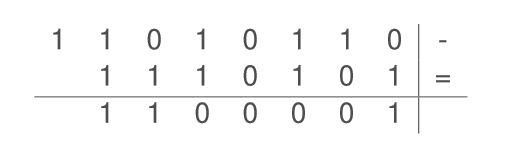
\includegraphics[width=0.6\textwidth,keepaspectratio]{images/Sottrazione-Bin.png}
	\caption{Esempio di differenza}
\end{figure}

\paragraph*{Moltiplicazione} La moltiplicazione in base binaria si può semplificare con il metodo dello shifting, che è più facile illustrare con un esempio:  \begin{figure}[H]
	\centering
	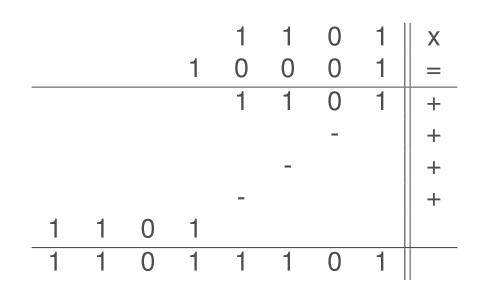
\includegraphics[width=0.6\textwidth,keepaspectratio]{images/Moltiplicazione-Bin.png}
	\caption{Esempio di prodotto}
\end{figure}
Si noti che quando è presente un 1 si riscrive il numero (nella posizione corrispondente) mentre  quando è presente uno 0 semplicemente non si scrive nulla (e si va solo avanti con le posizioni).

\subsection{Gli interi} Finora abbiamo visto come si codificano solo i numeri naturali, ma esistono metodi di codifica che permettono di rappresentare anche i numeri negativi (quindi l’insieme degli interi). Le tecniche più comuni sono: modulo e segno, complemento a 1 (\textit{CA1}) e complemento a 2 (\textit{CA2}).

\paragraph*{Codifica con Modulo e Segno:} Idea semplice: si usano $k-1$ bit per rappresentare il valore assoluto (modulo) del numero  ed un bit per codificare il segno (0=positivo, 1=negativo). In questo modo con k bit si possono codificare valori tra $-2^{k-1}+1 \text{ e} +2^{k-1}-1$.\\
\underline{N.B.}: esistono due codifiche per lo $0$, $-0$  e $+0$, e questo è un spreco.

\paragraph*{Codifica in Complemento a 1:} L’idea alla base è semplice, il primo bit indica sempre il segno e per ottenere l’opposto di un numero positivo si invertono tutti gli 0 in 1 e gli 1 in 0 (e lo stesso si fa per ottenere l’opposto di un numero negativo). Si hanno ancora due rappresentazioni per +0 e -0. È più facile da sommare rispetto al modulo e segno ma solo se il bit significativo non da riporto.
Quando si sommano due numeri in \textit{CA1}:
\begin{figure}[H]
	\centering
	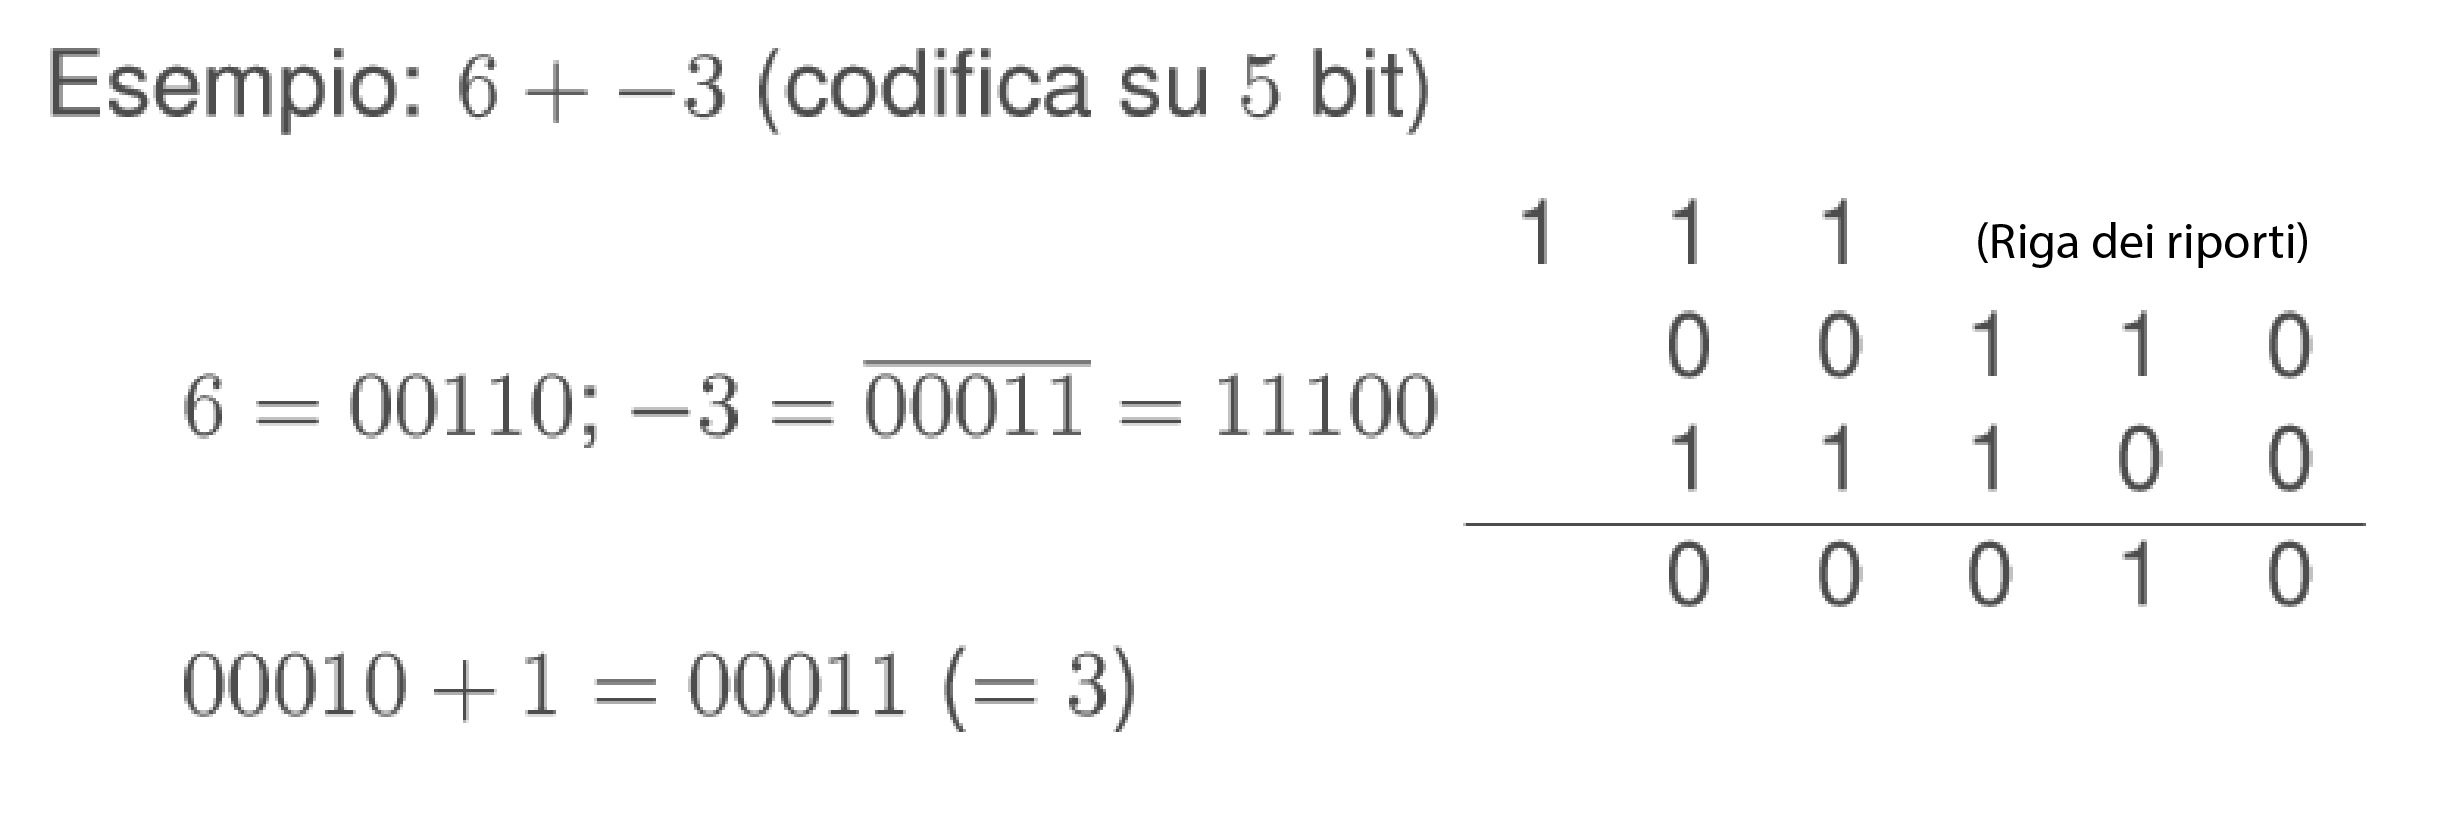
\includegraphics[width=0.9\textwidth,keepaspectratio]{images/Somma-CA1.png}
	\caption{Esempio di somma in CA1}
\end{figure}
\begin{itemize}[noitemsep]
\item Si deve verificare che i riporti delle prime due cifre significative siano uguali, altrimenti il numero che si ottiene non è rappresentabile in CA1 su k bit.
\item Alla fine si deve sommare il riporto della prima cifra al risultato ottenuto (ultima riga).
\end{itemize}
\paragraph*{Codifica in Complemento a 2:} Per tradurre un numero da intero con segno a complemento a 2 (\textit{CA2}) basta invertire tutti i bit tranne quello di sego e poi aggiungere 1. Viceversa per convertire da \textit{CA2} a binario con segno si sottrae 1 e poi si invertono tutti i bit tranne quello di segno. \\
Ancora una volta il bit più significativo indica il segno, ma in questo caso la codifica dello 0 è unica, quindi con \textit{k} bit si possono rappresentare i numeri da $-2^{k-1}$ a $2^{k-1}-1$. Anche la somma è più semplice ma questo lo vedremo in futuro.

